\documentclass[a4paper,12pt]{article}

%%% Поля
\usepackage[
    left=2cm,
    right=2cm,
    top=2cm,
    bottom=3cm,
    bindingoffset=0cm
]{geometry}

%%% Работа с русским языком
\usepackage{cmap}                       % поиск в PDF
\usepackage{mathtext}                   % русские буквы в формулах
\usepackage[T2A]{fontenc}               % кодировка
\usepackage[utf8]{inputenc}             % кодировка исходного текста
\usepackage[english,russian]{babel}     % локализация и переносы
\usepackage{indentfirst}
\frenchspacing

%%% Дополнительная работа с математикой
\usepackage{amsmath,amsfonts,amssymb,amsthm,mathtools}  % AMS

%%% Текст в колонки
\usepackage{multicol}

%%% Списки
\usepackage{enumitem}
\setlist{nosep, leftmargin=*}
\renewcommand{\labelenumi}{\arabic*)}

%%% Системы уравнений
\usepackage{cases}

%%% Таблицы
\usepackage{array}
\usepackage{makecell}

%%% Рисунки
\usepackage{graphicx}
\usepackage{float}

%%% Точка в подписях к рисункам
\usepackage[labelsep=period]{caption}

%%% Список литературы
\usepackage[
    natbib = true,
    style = alphabetic,
    sorting = none,
    backend = biber,
    language = autobib,
    autolang = other
]{biblatex}
\addbibresource{references.bib}

%%% Исправление символа номера при использовании gost-numeric.bbx
\usepackage{textcomp}
\DefineBibliographyStrings{russian}{number={\textnumero}}

%%% Гиперссылки
\usepackage[pdftex,unicode]{hyperref}

%%% Перенос знаков в формулах (по Львовскому)
\newcommand*{\hm}[1]{#1\nobreak\discretionary{}{\hbox{$\mathsurround=0pt #1$}}{}}


%%% Свои команды

\newcommand{\forcehyphenation}{-\linebreak}

\newcommand{\absent}[1]{[...#1...]}


%%% Заглавие
\title{Классификация русских классических стихов \\ по эпохам}
\author{Пономарев Андрей Сергеевич}
\date{2024--2025 учебный год, \\ весенний семестр}


\begin{document}
\maketitle

\begin{abstract}
    Настоящая работа посвящена применению современных средств обработки естественного языка для анализа русских стихотворных текстов. Решается задача классификации русской классической поэзии по эпохам. Для задачи составлен и размечен датасет. Обучены две модели: LSTM-нейросеть, использованная с готовыми эмбеддингами, а также классификатор на основе кодировщика RuBERT-tiny2. Второй показывает точность около $70 \%$.

    Репозиторий проекта находится по ссылке \\
    \url{https://github.com/ponomarevandr/russian_poems_classification}.
\end{abstract}



\section{Введение}

Обработка естественного языка (natural language processing)~-- область информатики, в настоящее время переживающая бурное развитие. Ее методы находят широкое применение в самых разных прикладных задачах. Из-за подобной широты многие задачи все еще далеки от исчерпывающего анализа, существующие решения можно свободно дорабатывать и развивать.

Одним из разделов обработки естественного языка, которые поныне не находятся в центре внимания, является анализ стихотворных текстов. Об этом свидетельствует как относительно малое число публикаций по теме, так и слова их авторов напрямую (например, \cite{barbado2021}).

В настоящем проекте предлагается решение задачи классификации русских классических стихотворений по эпохе, или, иначе, течению, направлению. Автор не нашел в Интернете статей, освещавших бы в точности этот вопрос, и в этом смысле работа нова.

Будут рассмотрены два подхода к решению задачи: с помощью нейронной сети LSTM (в качестве базового) и с помощью предобученной модели RuBERT-tiny2.

Лучший результат показала модель RuBERT-tiny2~-- точность около $70 \%$. Она в дальнейшем может применяться на практике, например, для категоризации стихотворений в Интернете, как классических, так и современных.


\subsection{Команда}

Проект подготовил \textbf{Пономарев А. С.}


\section{Смежные работы}

Перечислим несколько статей, близких проекту по тематике.

Работа \cite{noraini2012} посвящена классификации малайской поэзии по нескольким темам. Статья написана давно и использует ныне устаревший подход~-- метод опорных векторов (SVM) поверх TF-IDF,~-- но подходит для знакомства с задачей.

Интересна и обширна статья \cite{ruma2022}. Авторы рассматривают задачу классификации стихотворений Хафиза Ширази (на персидском языке) по периодам в жизни автора, что совсем близко к теме настоящего проекта. Основная используемая модель~-- LSTM-нейросеть, но помимо нее авторы пробуют логистическую регрессию, SVM, random forest, Bi-LSTM, GRU; в качестве эмбеддингов~-- CBOW, SkipGram, а также их конкатенацию. Авторы утверждают, что добились внушительной точности в $85 \%$.

Отметим также близкую по тематике работу \cite{orabi2020}, посвященную классификации арабской поэзии по эпохе написания. Авторы используют CNN-нейросеть с эмбеддингами FastText, относительно большой датасет (десятки тысяч стихотворений) и получают точность порядка $80 \%$.

В работе \cite{barbado2021} исследуется применение моделей-трансформеров для разбиения испанских сонетов по категориям выражаемых чувств. Для различных классов авторы добиваются F1-метрики от $0.6$ до $0.8$.

В отдельную ветвь можно выделить исследования, приспосабливающие для анализа стихотворных текстов предобученные BERT-подобные модели. В работе \cite{shahriar2023} дообучена модель AraBERT для классификации арабской поэзии по выражаемым эмоциям (точность $76.5 \%$). Статья \cite{rosa2023} описывает масштабный труд по обучению модели ALBERTI~-- мультиязыкового кодировщика для анализа стихотворений~-- на огромном массиве данных в миллионы произведений. Авторы утверждают, что на момент создания как сама модель, так и показанные результаты не имели аналогов. В работе также затронута интересная тема анализа средствами машинного обучения метрики стиха (то есть рисунка слогов и ударений).


\section{Данные}

Для работы с моделями был создан и размечен датасет русской классической поэзии. За основу взяты два ранее существовавших датасета стихов, размещенные в открытом доступе: \cite{russian_poetry_corpus} и \cite{russian_poems_19000}.

После объединения исходных датасетов данные были приведены к единому формату и очищены (см. Юпитер-тетрадку \textit{dataset\_preparation.ipynb}). Итоговая структура датасета показана в таблице \ref{tab:dataset}.

\begin{table}[t]
\centering
\begin{tabular}[t]{|m{1.4cm}|m{2.8cm}|m{4.2cm}|m{2.9cm}|m{1.3cm}|m{1.4cm}|}
    \hline
    & \textbf{author} & \textbf{epoch} & \textbf{title} & \textbf{part} & \textbf{text} \\
    \hline
    \hline
    Содер\-жание & \makecell[l]{Фамилия \\ автора} \par & \makecell[l]{Эпоха (течение, \\ направление)} \par & Заглавие & Номер фрагмента & Текст фрагмента \\
    \hline
    Формат & Русские буквы: заглавная, далее строчные; дефис & \makecell[l]{Одно из: \\ классицизм, \\ золотой век, \\ критический реализм, \\ серебряный век, \\ футуризм, \\ соцреализм, \\ шестидесятники} \par & Строчные русские и~английские буквы, цифры, пробел & Индекс с нуля & $8$--$40$ строк, без пустых строк \\
    \hline
\end{tabular}
\caption{Структура датасета.}
\label{tab:dataset}
\end{table}

Поле \textit{author} всюду приведено к одной лишь фамилии автора; в случае совпадений используются приписки через дефис, например: \textit{Багрицкий-отец}, \textit{Иванов-В}. Исключены иноязычные авторы, представленные в переводах.

Заглавие в поле \textit{title} приведено к нижнему регистру и очищено ото всех небуквенных символов, кроме цифр и пробелов.

В текстах стихотворений по возможности исправлены ошибочные символы, удалены теги, сноски, номера строф, символьные артефакты. Убраны пустые строки. Исключены записи, состоящие преимущественно не из русских букв или имеющие среднюю длину строки более $60$ символов.

Из датасета удалены дубликаты. Их поиск велся как по заглавию, так и по расстоянию Левенштейна между текстами.

При работе с моделью было решено использовать стихотворные тексты длиной от $8$ до~$40$ строк включительно. Для этого все более длинные произведения были <<нарезаны>> на фрагменты допустимой случайной длины. Эмпирически установлено, что распределение длин коротких стихотворений в строках близко к гамма-распределению, $\xi \sim \text{Gamma}(\alpha, \beta)$, с матожиданием $\text{E} \xi \approx 18.23$ и дисперсией $\text{D} \xi \approx 81.66$. Напомним, что его плотность определяется формулой
\[
    p_{\alpha, \beta}(x) = \cfrac{\beta^\alpha x^{\alpha - 1} e^{-\beta x}}{\Gamma(\alpha)},
\]
а также верно $\text{E} \xi = \alpha / \beta$ и $\text{D} \xi = \alpha / \beta^2$. Случайные длины при разбиении стихотворений на фрагменты получались округлением элементов выборки из описанного распределения.

Поле \textit{epoch} является целевым признаком. Будем называть его эпохой стихотворения (синонимы: течение, направление). Выделим семь основных эпох: см. таблицу \ref{tab:epoches}. Каждая эпоха имеет своеобразные черты и примерную датировку, представление о которых дают многочисленные открытые источники. Однако автору неизвестно единого исследования, которое давало бы исчерпывающее и достаточно строгое разбиение русской поэзии по эпохам, поэтому он в немалой степени руководствовался личной интуицией и чувством прекрасного.

\begin{table}[t]
\centering
\begin{tabular}[t]{|m{3.4cm}|m{3.6cm}|m{8cm}|}
    \hline
    Эпоха & \makecell[l]{Примерная \\ датировка} & Комментарий \\
    \hline
    \hline
    Классицизм & XVIII век & \\
    \hline
    \makecell[l]{Золотой век \\ русской поэзии} & Первая половина XIX века & \\
    \hline
    \makecell[l]{Критический \\ реализм} & Вторая половина XIX века & Близко к понятию <<натуральной школы>> \\
    \hline
    \makecell[l]{Серебряный век \\ русской поэзии} & Начало XX века & Близко к понятию символизма \\
    \hline
    Футуризм & Начало XX века & Может рассматриваться как часть Серебряного века, но резко выделяется и достаточно объемен \\
    \hline
    Социалистический реализм & Середина XX века & \\
    \hline
    \makecell[l]{Поэзия \\ шестидесятников} & Вторая половина XX века & \\
    \hline
\end{tabular}
\caption{Эпохи, выделяемые в русской поэзии.}
\label{tab:epoches}
\end{table}

Для простоты будем считать, что эпоха стихотворения определяется эпохой его автора; $189$ авторам, представленным в датасете, были присвоены метки в соответствии со сказанным выше, а затем перенесены на соответствующие фрагменты произведений. Списки авторов по эпохам см. в Юпитер-тетрадке \textit{dataset\_labeling.ipynb}.

Получившееся разбиение на классы относительно сбалансированно: самый большой~-- Серебряный век~-- содержит $16204$ стихотворных фрагмента; самый малый~-- шестидесятники~-- $3238$, что примерно в $5$ раз меньше, и сразу за ним~-- классицизм~-- $3281$. 

Для работы с моделями датасет разбивался на три части: тренировочную (train), валидационную (eval) и тестовую (test)~-- в соотношении $70:15:15$.


\section{Модели}

\subsection{LSTM}

Первая использованная модель, и она же взятая в качестве базового решения (base\-line),~-- это нейронная сеть типа Long short-term memory (LSTM) (см. Юпитер-тетрадку \textit{training\_lstm.ipynb}). Для работы выбрана известная реализация из библиотеки Pytorch~-- класс \textit{nn.LSTM}. Поверх стандартной LSTM-нейросети добавлен полносвязный линейный слой (\textit{nn.Linear}) с функцией активации LogSoftmax для получения логарифмированных вероятностей классов.

Для кодирования текста используются готовые русскоязычные эмбеддинги \textit{word2vec-ruscorpora-300} из библиотеки Gensim. Для их работы требуется лемматизация и определение части речи; то и другое производится средствами библиотеки Pymorphy3 пословно.

Нейросеть \textit{nn.LSTM} имеет размерность входа $300$, размерность внутреннего состояния $400$ и единственный скрытый слой.

Для обучения использовался оптимизатор \textit{optim.Adam} с параметром $lr = 1.5 \cdot 10^{-4}$ (learning rate).

\begin{figure}[tp]
    \centering
    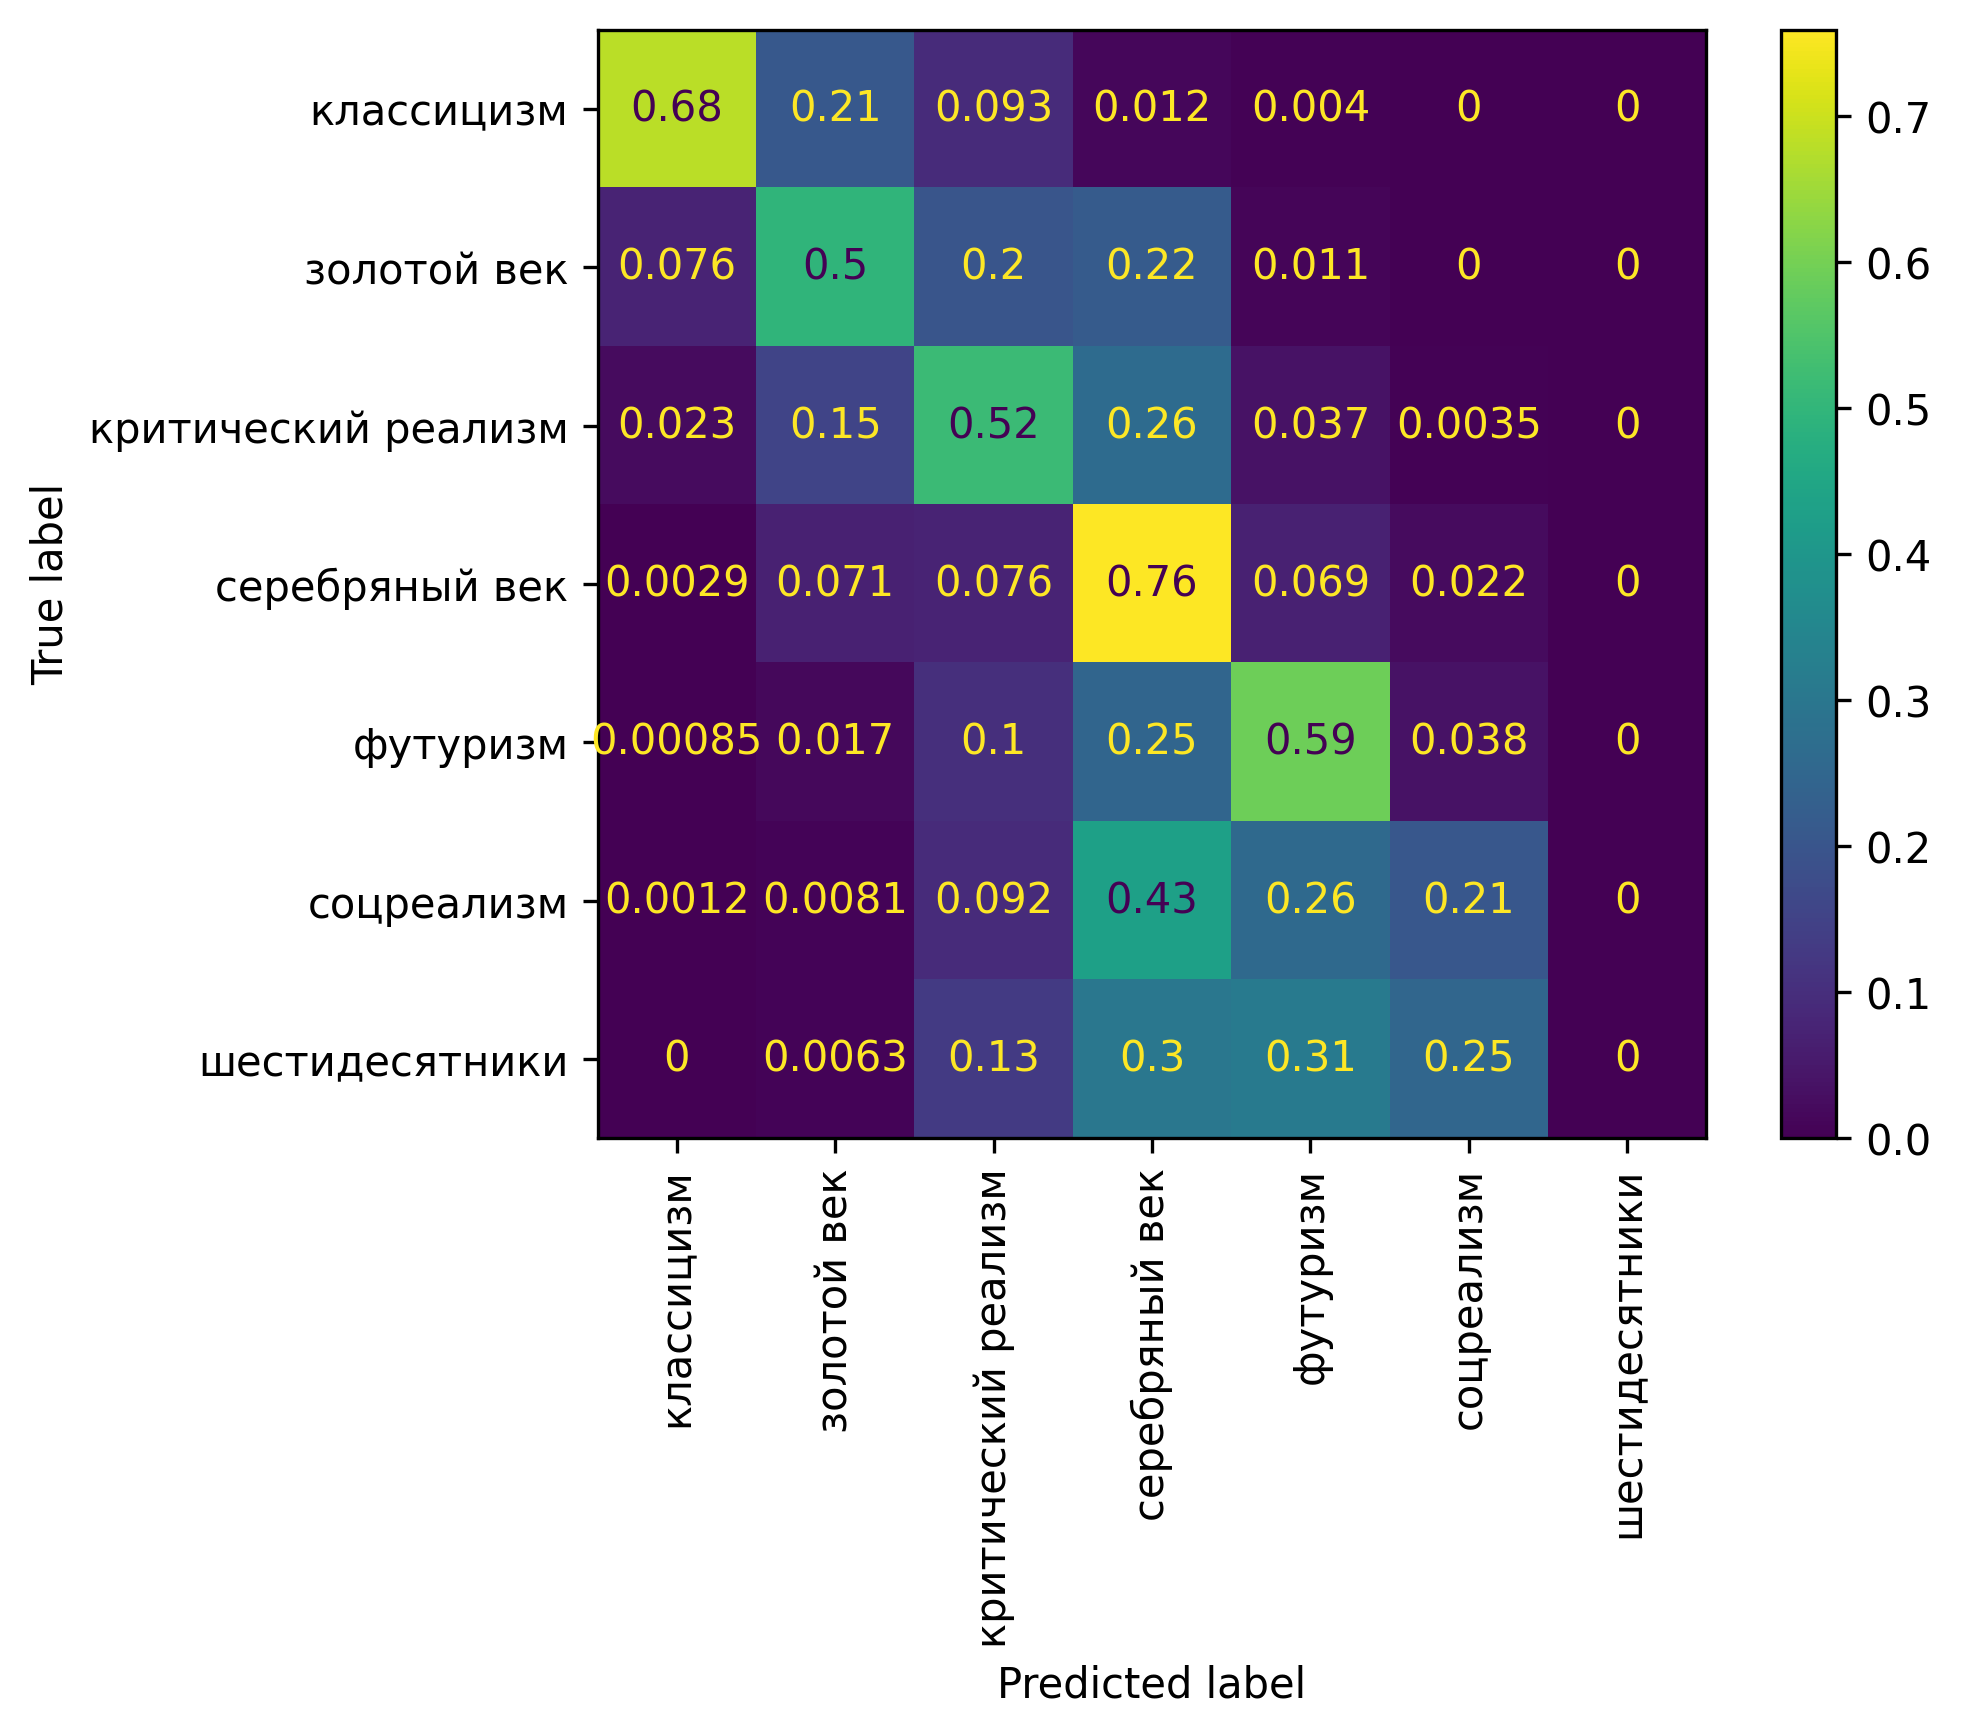
\includegraphics[width=0.75\linewidth]{figures/lstm_confusion_matrix.png}
    \vspace{-0.3cm}
    \caption{Матрица ошибок LSTM-модели.}
    \label{fig:lstm_confusion}
    \vspace{0.5cm}
    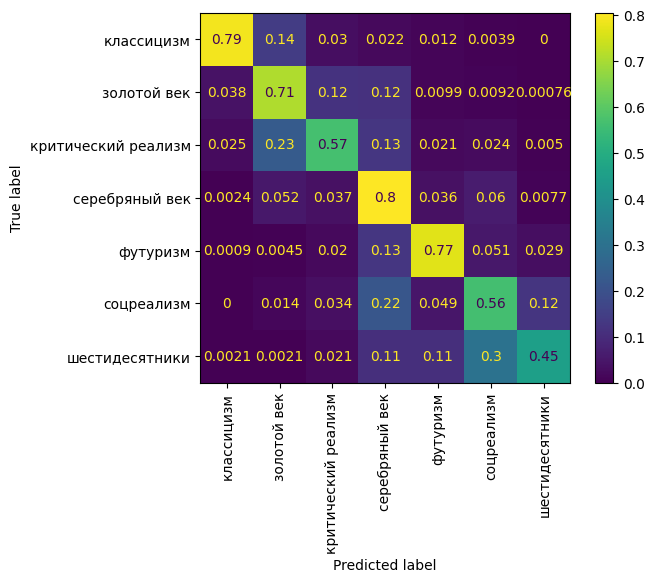
\includegraphics[width=0.75\linewidth]{figures/rubert_confusion_matrix.png}
    \vspace{-0.3cm}
    \caption{Матрица ошибок модели RuBERT-tiny2.}
    \label{fig:rubert_confusion}
\end{figure}


\subsection{RuBERT-tiny2}

Вторая использованная модель~-- это BERT-подобный кодировщик RuBERT-tiny2 (см. Юпитер-тетрадку \textit{training\_rubert.ipynb}), опубликованный в Интернете \cite{rubert_model}. Модель была выбрана, во-первых, потому, что специально предназначена для русскоязычных текстов, во-вторых, из-за своего сравнительно малого (как и обещает название) размера в $29.4$ миллиона параметров.

Работа с моделью происходит через библиотеки Datasets, Evaluate и Transformers компании Hugging Face. Автор значительно опирался на код из Юпитер-тетрадки \cite{rubert_notebook}. Хотя исходно модель RuBERT-tiny2~-- это кодировщик, а не классификатор, средства библиотек позволяют загрузить ее в класс \textit{AutoModelForSequenceClassification}, автоматически добавляя необходимые элементы. Для обучения использовался оптимизатор \textit{optim.Adam} из библиотеки Pytorch, с параметром $lr = 10^{-5}$. Модель поддерживает работу на GPU (Cuda), что значительно ускорило обучение~-- средствами Google Colab оно было завершено приблизительно за 25 минут.


\section{Результаты}

Предсказания моделей оценены по двум стандартным метрикам: accuracy (точности) и weighted F1 -- результаты в таблице \ref{tab:results}.

\begin{table}[t]
\centering
\begin{tabular}[t]{|l|c|c|}
    \hline
    Модель & accuracy & weighted F1 \\
    \hline
    LSTM-нейросеть & 0.543 & 0.514 \\
    RuBERT-tiny2 & 0.696 & 0.694 \\
    \hline
\end{tabular}
\caption{Результаты моделей на тестовых данных.}
\label{tab:results}
\end{table}

Для полученных на тестовых данных предсказаний также построены матрицы ошибок (confusion matrices), см. рис. \ref{fig:lstm_confusion}, \ref{fig:rubert_confusion}.

LSTM-модель показала удовлетворительный результат. Она справляется с задачей примерно в половине случаев; притом никогда не выдает в качестве результата поэзию шестидесятников.

Дообученная модель RuBERT-tiny2 справляется с задачей хорошо, демонстрируя значительную точность примерно в $70 \%$. Наиболее трудны для определения оказываются опять же шестидесятники, за ними~-- соцреализм и критический реализм. Легче всего оказывается распознать поэзию Серебряного века и классицизма. Заметим, что трудность определения обусловлена вовсе не только размерами классов.


\section{Файлы моделей и демонстрация работы}

Файлы обеих обученных моделей сохранены в репозитории. В Юпитер-тетрадке \linebreak \textit{training\_rubert.ipynb} приведен минимальный код, открывающий файлы готовой модели и позволяющий запустить ее на любом тексте по желанию пользователя.


\section{Заключение}
\begin{itemize}
    \item Составлен датасет русских классических стихотворений. Датасет размечен: добавлен целевой признак эпохи (течения, направления), всего $7$ классов.
    \item Для решения задачи классификации обучена LSTM-нейросеть, использовавшаяся вместе с готовыми русскоязычными эмбеддингами. Модель показала удовлетворительный результат: точность порядка $50 \%$.
    \item Для решения задачи классификации применена предобученная модель RuBERT-tiny2, основные достоинства которой~-- приспособленность к русскому языку и сравнительно малый размер. Дообученная модель показала хороший результат на тестовых данных: точность около $70 \%$.
    \item Полученная на основе RuBERT-tiny2 модель может в дальнейшем использоваться на практике, например, для категоризации стихов на интернет-сайтах.
\end{itemize}


\begin{otherlanguage}{english}
\printbibliography[
    heading=bibintoc
]
\end{otherlanguage}

\end{document}